% !TeX spellcheck = en_US
% !TeX root = ./0_article.tex

\section{Body biasing injection platforms modeling}
\IEEEPARstart{T}{he} objective of this first section is to present the work done concerning electrical modeling of integrated circuits in a BBI context.
Developing IC models in that specific case is not an easy task.
Indeed, modern digital ICs contains billions of transistors, and even considering microcontrollers where the transistor count is less important, with current technologies, it is impossible to evaluate circuits at a transistor level.

\subsection{The hybrid simulation flow}
To tackle these limitations, we decided to adopt an hybrid approach, combining transistor-less models and local logic gates simulations.
This approach allows simulating relatively big circuits under BBI disturbances.
To that end, the whole simulation flow was divided in three consecutive steps:
\begin{itemize}
	\item The simulation of an IC under BBI using a transistor-less model, allowing for a purely electrical analysis;
	\item The extraction of significant disturbed signals from the previous simulation;
	\item The simulation of functional logic gates under BBI thanks to the previously extracted signals.
\end{itemize}
The first step allows analyzing IC macro-electrical behavior when subject to BBI, and at a lower computational cost compared to a functional model including transistors and internal transmission lines, even if it could be done in a reasonable time constraint for millions of transistors.
Then, by extracting useful signals such as the power delivery and the transistor substrate voltages, we can evaluate what would be the behavior of actual logic gates subject to BBI.

%Therefore, and as it has been proposed in \textcolor{cyan}{FDTC2022 and FDTC2023}, we approach the problem using transistor-less models.
\subsection{The standard-cell model}
The transistor-less model, also called standard-cell model, is developed thanks to the internal structure of integrated circuits, including:
\begin{itemize}
	\item Their power supply network;
	\item Their standard-cells properties;
	\item Their silicon substrate.
\end{itemize}
These three elements and their internal structure allow elaborating average models, able to represent their macro behavior.
Fig. \ref{fig_alim_std} illustrates the base symbolic diagram used for our design.
It represents a standard-cell segment, composed of logic gates and decoupling elements, with a fixed height of 5 µm and a variable width.
Two levels of metals for the power distribution are represented, the highest level MTOP in green and the first level M1 in blue.

Then, 

%\IEEEPARstart{W}{hen} studying integrated circuits in a fault injection context, it is often required to elaborate electrical models.
%They allow simulating parts or entire circuits subjected to BBI, therefore acquiring insights on the mechanisms at work.
%The acquired knowledge allows to set up more reliable experiments as well as countermeasures.
%
%In this context, we developed, thanks to previous works on the subject \textcolor{cyan}{Citations ICI}, electrical models

% !TeX spellcheck = en_US
% !TeX root = ./0_article.tex

\begin{figure}[h]
	\label{fig_alim_std}
	\centering
	\includegraphics[width=0.49\textwidth]{./figures/psu_std_cell.pdf}
	\caption{A Standard-Cell Segment and its power delivery network.}
\end{figure}


% !TeX spellcheck = en_US
% !TeX root = ./0_article.tex

\begin{figure}[h]
	\centering
	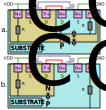
\includegraphics[width=0.35\textwidth]{./figures/substrate_2.pdf}
	\caption{Triple-well (a) and Dual-well (b) inverter cross-sectional view.}
	\label{fig_sub}
\end{figure}


% !TeX spellcheck = en_US
% !TeX root = ./0_article.tex

\begin{figure*}[ht]
	\centering
	\includegraphics[width=1.0\textwidth]{./figures/dual+triple3.png}
	\caption{Triple well (left) and dual well (right) std cell}
	\label{fig_triplewellstdcell}
\end{figure*}


%\IEEEPARstart{T}{his} section approaches the electrical modeling of BBI platforms and integrated circuits.
%As it has been proposed in \textcolor{cyan}{Cosade2022Chancel, FDTC2022\&2023Chancel}, it is possible to model BBI ICs using transistor-less models.
%It has the advantage of providing a somewhat precise evaluation of the mechanisms at work, while allowing for large simulations in reasonable times.
%Within this context, we decided